\documentclass{llncs}
\pagestyle{plain}

%\usepackage[latin9]{inputenc}
%\usepackage[T1]{fontenc}
\usepackage{float}
\usepackage{wrapfig}
\usepackage{amsmath}
\usepackage{amssymb}
\usepackage{graphicx}
\usepackage{tikz}
\usepackage{tikz-3dplot}
\usepackage{subcaption}
\usepackage{tabularx}
\captionsetup{compatibility=false}
% \usepackage{esint}
\usepackage{array}
\usepackage{epstopdf}
\usepackage{placeins}
\usepackage{pgfplots}
\usepackage{url}
\usepackage{tikz}
\usepackage{calc}
\usepackage[linesnumbered,ruled,vlined]{algorithm2e}
\usetikzlibrary{positioning, arrows.meta,calc}
%%%%%%%%%%%%%%%%%%%%%%%%%%%%%%%
%%%%%%%%%%%%%%%%%%%%%%%%%%%%%%%
\newcommand{\vx}{\boldsymbol{x}}
\newcommand{\vy}{\boldsymbol{y}}
\newcommand{\vW}{\boldsymbol{W}}
\newcommand{\vz}{\boldsymbol{z}}
\newcommand{\vb}{\boldsymbol{bias}}
\newcommand{\val}{{\textrm{value}}}
\newcommand{\Val}{{\textrm{value}}}
\newcommand{\MILP}{{\textrm{MILP}}}
\newcommand{\LP}{{\textrm{LP}}}

\newcommand{\UB}{\mathrm{UB}}
\newcommand{\LB}{\mathrm{LB}}
\newcommand{\ub}{\mathrm{ub}}
\newcommand{\lb}{\mathrm{lb}}
\newcommand{\B}{\mathrm{B}}

\newcommand{\CMP}{{\textrm{CMP}}\ }


\newcommand{\toolname}{\CMP}






%\usepackage{amsmath, amsthm, amssymb, amsfonts}
%\newtheorem{theorem}{Theorem}
%\newtheorem{lemma}{Lemma}
%\newtheorem{corollary}{Corollary}
%\theoremstyle{definition}
%\newtheorem{definition}{Definition}



\newcommand{\ReLU}{\mathrm{ReLU}}



\title{Liptschiz}
\date{}

\begin{document}
	
	\maketitle
	
	\begin{abstract}
		
		Local robustness is bad. We study a more global notion, lipsitcz constant.
		
	\end{abstract}
	
	
	\section{Introduction}
	
	TO DO.
	
	\section{Notations and Preliminaries}
	
	In this paper, we will use lower case latin $a$ for scalars, bold for vectors $\boldsymbol{z}$, 
	capitalized bold for matrices $\boldsymbol{W}$, similar to notations in \cite{prima,crown}.
	To simplify the notations, we restrict the presentation to feed-forward, 
	fully connected ReLU Deep Neural Networks (DNN for short), where the ReLU function is $ReLU : \mathbb{R} \rightarrow \mathbb{R}$ with
	$ReLU(x)=x$ for $x \geq 0$ and $ReLU(x)=0$ for $x \leq 0$, which we extend componentwise on vectors.
	
	%In this paper, we will not use tensors with a dimension higher than matrices: those will be flattened.
	
	%\subsection{Neural Network and Verification}
	
	
	% testtesttesttest
	An $\ell$-layer DNN is provided by $\ell$ weight matrices 
	$\boldsymbol{W}^i \in \mathbb{R}^{d_i\times d_{i-1}}$
	and $\ell$ bias vectors $\vb^i \in \mathbb{R}^{d_i}$, for $i=1, \ldots, \ell$.
	We call $d_i$ the number of neurons of hidden layer $i \in \{1, \ldots, \ell-1\}$,
	$d_0$ the input dimension, and $d_\ell$ the output dimension.
	
	Given an input vector $\boldsymbol{z}^0 \in \mathbb{R}^{d_0}$, 
	denoting $\hat{\boldsymbol{z}}^{0}={\boldsymbol{z}}^0$, we define inductively the value vectors $\boldsymbol{z}^i,\hat{\vz}^i$ at layer $1 \leq i \leq \ell$ with
	\begin{align*}
		{\boldsymbol{z}}^{i} &= \boldsymbol{W}^i\cdot \hat{\boldsymbol{z}}^{i-1}+ \vb^i\\
		\hat{\boldsymbol{z}}^{i} &= ReLU({\boldsymbol{z}}^i).
	\end{align*} 
	
	The vector $\hat{\boldsymbol{z}}$ is called post-activation values, 
	$\boldsymbol{z}$ is called pre-activation values, 
	and $\boldsymbol{z}^{i}_j$ is used to call the $j$-th neuron in the $i$-th layer. 
	For $\boldsymbol{x}=\vz^0$ the (vector of) input, we denote by $f(\boldsymbol{x})=\vz^\ell$ the output. Finally, pre- and post-activation neurons are called \emph{nodes}, and when we refer to a specific node/neuron, we use $a,b,c,d,n$ to denote them, and $W_{a,b} \in \mathbb{R}$ to denote the weight from neuron $a$ to $b$. Similarly, for input $\boldsymbol{x}$, we denote by $\val_{\boldsymbol{x}}(a)$ the value of neuron $a$ when the input is $\boldsymbol{x}$. A path $\pi$ is a sequence $\pi=(a_i)_{k \leq  i \leq k'}$ of neurons in consecutive layers, and the weight of $\pi$ is 
	$weight(\pi)=W_{a_k,a_{k+1}} \times \cdots \times  W_{a_{k'-1},a_{k'}}$.
	
	
	
	\iffalse
	and the $i$-th hidden layer is a vector in $\mathbb{R}^{d_i}$, 
	and the output layer is a vector in $\mathbb{R}^{d'}$ or a scale. 
	The weights, bias and activation functions decide propagate the from previous to the next layer. In formula, from layer $l_{i-1}$ to layer $l_{i}$, the weight 
	$\boldsymbol{W}^i$ is matrix of $d_i\times d_{i-1}$, 
	the bias is a vector $\vb^i$ in $\mathbb{R}^{d_i}$, and the activation function 
	is $\sigma$, then  if the $i-1$-th layer is $\hat{\boldsymbol{z}}^{(i-1)}$, 
	then the value of $i$-th layer is computed by: 
	\begin{align*}
		{\boldsymbol{z}}^{i} &= \boldsymbol{W}^i\cdot \hat{\boldsymbol{z}}^{(i-1)}+ \vb^i\\
		\hat{\boldsymbol{z}}^{i}(n) &= \sigma({\boldsymbol{z}}^i(n)).
	\end{align*} The vector $\hat{\boldsymbol{z}}$ is called post-activation values, and $\boldsymbol{z}$ is called pre-activation values, and $\boldsymbol{z}^{(i)}_j$ is used to call the $j$-th neuron in the $i$-th layer. In our style, we also call neurons \emph{nodes} and use $a,b,c,d$ to denote them. We use $W_{ab}$ to denote the weight from neuron $b$ to $a$. We use $\boldsymbol{x}$ to denote the vector of input and  $f(\boldsymbol{x})$ to denote the output.
	\fi
	
	\medskip
	
	Concerning the verification problem, we focus on the well studied local-robustness question. Local robustness asks to determine whether the output of a neural network will be affected under small perturbations to the input. 
	Formally, for an input $\vx$ perturbed by $\varepsilon >0$ under distance $d$, then the DNN is locally $\varepsilon$-robust in $\vx$ whenever:
	\begin{align*}
		\forall \boldsymbol{x'} \text{ s.t. } d(\vx,\vx')\leq \varepsilon, \text{ we have }  
		argmax_i (f(\boldsymbol{x'})[i]) = argmax_i(f(\boldsymbol{x})[i])
	\end{align*} 
	
	\iffalse
	In some cases, the output is a vector but the aim to get the label of dimension with the minimal value. In this case, the problem can be written as:\begin{align*}
		\forall \boldsymbol{x} \in\mathcal{D} \  \min f(\boldsymbol{x}) = \min f(\boldsymbol{x}_0)
	\end{align*}
	
	If so, the question of verification can turn to the following optimization question: \begin{align*}
		\min f(\boldsymbol{x}) \ s.t. {\boldsymbol{z}}^{i} &= \boldsymbol{W}^i\cdot \hat{\boldsymbol{z}}^{(i-1)}+ b^i\\
		\hat{\boldsymbol{z}}^{i}(n) &= \sigma({\boldsymbol{z}}^i(n)), \boldsymbol{x}\in\mathcal{D}.
	\end{align*}
	
	In this paper, we only consider $\ReLU$ function as the activation function: $\sigma(a)=\ReLU(a)=\max(0,a)$. 
	
	In this paper, we consider $L^{\infty}$ norm the max value of distance of each dimension, that is $d(\vx,\boldsymbol{x}_0)=\max |\boldsymbol{x}(n)-\boldsymbol{x}_0(n)|$. 
	\fi
	
	

	\section{Value Abstraction for DNN verification}

In this section, we describe different value (over-)abstractions on $\vz$ that are used by efficient algorithms to certify robustness around an input $\vx$. Over-abstractions of values include all values for $\vz$ in the neighbourhood of $\vx$, and thus a certificate for safety in the over-abstraction is a proof of safety for the original input $\vx$.

\subsection{The Box and DeepPoly Abstractions}



\begin{figure}[t!]
	\centering
	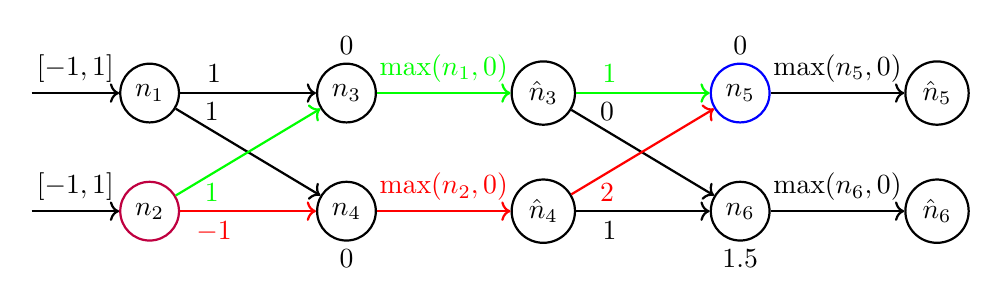
\begin{tikzpicture}
		
		\node[circle, draw= black, thick, minimum width = 20,
		minimum height = 20] (input1) {$n_1$};
		
		\node[circle, draw= purple, thick, minimum width = 20,
		minimum height = 20] (input2) at ($(input1) + (0,-1.5)$) {$n_2$};
		
		
		% Hidden layers
		
		\node (hidden10) at ($(input1) + (2.5,0.6)$) {$0$};
		
		\node (hidden20) at ($(input1) + (2.5,-1.5-0.6)$) {$0$};
		
		\node (hidden50) at ($(input1) + (7.5,0.6)$) {$0$};
		
		\node (hidden60) at ($(input1) + (7.5,-1.5-0.6)$) {$1.5$};
		
		
		\node[circle, draw= black, thick, minimum width = 20,
		minimum height = 20] (hidden1) at ($(input1) + (2.5,0)$) {$n_3$};
		\node[circle, draw= black, thick] (hidden2) at ($(input1) + (2.5,-1.5)$) {$n_4$};
		
		\node[circle, draw= black, thick, minimum width = 20,
		minimum height = 20] (hidden3) at ($(input1) + (5,0)$){$\hat{n}_3$};
		\node[circle, draw= black, thick] (hidden4) at ($(input1) + (5,-1.5)$) {$\hat{n}_4$};
		
		
		\node[circle, draw= blue, thick, minimum width = 20,
		minimum height = 20] (hidden5) at ($(input1) + (7.5,0)$){$n_5$};
		\node[circle, draw= black, thick] (hidden6) at ($(input1) + (7.5,-1.5)$) {$n_6$};
		
		
		
		
		% Output layer
		\node[circle, draw= black, thick, minimum width = 20,
		minimum height = 20] (output1) at ($(input1) + (10,0)$){$\hat{n}_5$};
		
		\node[circle, draw= black, thick, minimum width = 20,
		minimum height = 20] (output2) at ($(input1) + (10,-1.5)$){$\hat{n}_{6}$};
		
		
		% Connections
		
		\draw[->,thick] ($(input1) + (-1.5,0)$) -- (input1) node[midway, above] {$[-1,1]$};
		
		\draw[->,thick] ($(input1) + (-1.5,-1.5)$) -- (input2) node[midway, above] {$[-1,1]$};
		
		
		
		\draw[->,thick] (input1) -- (hidden1) node[near start, above] {$1$};
		\draw[->,thick] (input1) -- (hidden2)node[near start, above] {$1$};
		
		\draw[->,color=green, thick] (input2) -- (hidden1) node[near start, below] {$1$};
		\draw[->,color=red, thick] (input2) -- (hidden2)node[near start, below] {$-1$};
		
		
		
		
		
		\draw[->,color=green, thick] (hidden1) -- (hidden3) node[midway, above] {$\max(n_1,0)$};
		\draw[->,color=red, thick] (hidden2) -- (hidden4) node[midway, above] {$\max(n_2,0)$};
		
		
		
		
		
		\draw[->,color=green, thick] (hidden3) -- (hidden5) node[near start, above] {$1$};			
		\draw[->,thick] (hidden3) -- (hidden6) node[near start, above] {$0$};
		
		\draw[->,color=red, thick] (hidden4) -- (hidden5)node[near start, below] {$2$};
		\draw[->,thick] (hidden4) -- (hidden6)node[near start, below] {$1$};
		
		
		
		
		\draw[->,thick] (hidden5) -- (output1) node[midway, above] {$\max(n_5,0)$};
		\draw[->,thick] (hidden6) -- (output2) node[midway, above] {$\max(n_6,0)$};
		
		
	\end{tikzpicture}
	\caption{A DNN example from \cite{kpoly}: every neuron is separated into 2 nodes, $n$ pre- and $\hat{n}$ post-ReLU activation function. The pair $(n_2 n_3 n_5,n_2 n_4 n_5)$ in green and red is compensating (weights of paths are $1,-2$).}
	\label{fig1}
\end{figure}

The concept of value abstraction involves calculating upper and lower bounds for the values of certain neurons in a Deep Neural Network (DNN) when inputs fall within a specified range. This approach aims to assess the network's robustness without precisely computing the values for every input within that range.

Firstly, it's important to note that weighted sums represent a linear function, which can be explicitly expressed with relative ease. However, the ReLU (Rectified Linear Unit) function presents a challenge in terms of accurate representation. Although ReLU is a relatively straightforward piecewise linear function with two modes (one for $x<0$ and another for $x \geq 0$), it is not linear. The complexity arises when considering the compounded effects of the ReLU function across the various layers of a ReLU DNN. It's worth noting that representing $\ReLU(x)$ precisely is feasible when $x$ is "stable," meaning it's consistently positive or consistently negative, as there's only one linear mode involved in each scenario. Consequently, the primary challenge lies in addressing "unstable" neurons, where the linearity of the function does not hold consistently.


Consider the simpler abstraction, termed ``Box abstraction" \cite{deeppoly}: it inductively computes the bounds for each neuron in the subsequent layer independently. This is achieved by considering the weighted sum of the bounds from the previous layer, followed by clipping the lower bound at $\max(0,$ lower bound$)$ to represent the ReLU function, and so forth. For all $i$, define $x_i=\val_{\vx}(n_i)$, where $\vx=(x_1,x_2)$.

Taking the DNN example from Fig \ref{fig1}, assume $x_1,x_2 \in [-1,1]$. This implies that $x_3,x_4 \in [-2,2]$. After applying the ReLU function, $\hat{x}3,\hat{x}4$ are constrained to $[0,2]$, leading to $x_5 \in [0,6]$ and $x_6 \in [0,2]$. The bounds for $n_1, \ldots, n_4$ are exact, meaning for every $\alpha$ within the range, an input $\vy$ can be found such that $\val{\vy}(n_i)=\alpha$. However, this precision is lost from the next layer (beginning with $n_5, n_6$) due to potential dependencies among preceding neurons. For example, $n_3$ only attains the value $2$ when both $x_1$ and $x_2$ are $2$. In this case, $n_4$ would reach a value of $Val{(2,2)}(n_4)=0$. Consequently, it's implausible for $x_5=\Val_{\vx}(n_5)$ to reach $6$, as it would necessitate both $n_3$ and $n_4$ assuming the value $2$.

An extremely efficient algorithm that addresses some issues is "DeepPoly" \cite{deeppoly}, also independently discovered as the "CROWN" algorithm \cite{crown}. Instead of strict bounds, for each neuron $n$ in layer $k$, DeepPoly maintains two affine functions representing the lower and upper bounds of the neuron's value, based on inputs from the previous layer $k-1$. For instance, denote $f_i \leq x_i \leq g_i$ with, for example, $f_{3}(x_3)=f_4(x_4)=0$ and $g_3(x_3) = \frac{x_3+2}{2}$, $g_4(x_4) = \frac{x_4+2}{2}$. This leads to $x_5 \leq g_3(x_3) + 2 g_4(x_4) = \frac{x_3 + 2x_4 + 6}{2} = \frac{3x_1 - x_2 + 6}{2}\leq 5$.

For bounds $[\alpha,\beta]$ on $x_i$, the optimal linear function for the upper bound is $g_i(x_i)= \beta \frac{x_i-\alpha}{\beta-\alpha}$ for ReLU nodes. There are two options for the lower bound: $f^1_i(x_i) = 0$ or $f^2_i(x_i)=x_i$. DeepPoly selects between these based on the values of $\alpha$ and $\beta$ (for unstable neurons): if $|\alpha|\geq |\beta|$, then $f_i=f^1_i$ is chosen, otherwise, for $|\beta|>|\alpha|$, $f_i=f^2_i$ is selected. The variation, {\em $\overline{\mbox{DeepPoly}}$}, consistently chooses $f^1_i$, and never $f^2_i$. Contrary to DeepPoly, {\em $\overline{\mbox{DeepPoly}}$} encompasses the ``Box abstraction." For instance, with bounds $[-0.2,5]$ on $x_i$, it deduces $\ReLU(x_i) \in [0,5]$, whereas  DeepPoly without box abstraction algorithm would conclude $\ReLU(x_i) \in [-0.2,5]$.


\iffalse
\subsection{PRIMA and $\beta$-CROWN}
\fi

\subsection{MILP and LP encodings for DNNs}

At the other end of the spectrum, we find the Mixed Integer Linear Programming (MILP) value abstraction, which is a priori a complete method (albeit much slower than DeepPoly). 
Consider an unstable neuron $n \in[\alpha,\beta]$. The value $x$ of $\ReLU(n)$ can be encoded exactly in an MILP formula with one integer (actually even binary) variable $a$ valued in ${0,1}$, using 4 constraints \cite{MILP}:
\vspace{-0.1cm}
\begin{align*}
	\hat{x} \geq x \quad \wedge \quad \hat{x} \geq 0, \quad \wedge \quad \hat{x} \leq \beta \cdot a \quad \wedge \quad \hat{x} \leq x-\alpha \cdot (1-a)
\end{align*}

It can be shown that for all $x \in [\alpha,\beta] \setminus 0$, there exists a unique solution $(a,\hat{x})$ that meets these constraints, with $\hat{x}=\ReLU(x)$. Here, $a$ is 0 if $x < 0$, 1 if $x>0$, and can be either if $x=0$~\cite{MILP}. This encoding approach can be applied to every (unstable) ReLU node, and optimizing its value can help in certifying a given input. However, for networks with hundreds of nodes or more, the resulting MILP formulation will contain numerous integer variables and generally cannot be solved efficiently.

MILP instances can be linearly relaxed into LP over-abstraction, where variables originally restricted to integers in ${0,1}$ (binary) are relaxed to real numbers in the interval $[0,1]$, while maintaining the same encoding. As solving LP instances is polynomial time, this optimization is significantly more efficient. However, this efficiency comes at the cost of precision, often resulting in less stringent bounds. This approach is termed the {\em LP abstraction}

The following proposition shows that the LP abstraction refines the DeepPoly abstraction. 
The difference between the LP and the DeepPoly abstractions is that LP simultaneous considers the two linear lower bounding functions for the ReLU operation, namely $ReLU(x) \geq 0$ and $ReLU(x) \geq x$, while the DeepPoly abstraction restricts itself to the application of a single one of these linear bounding functions.
 

\begin{proposition}
	\label{LP}
	Given $x \in [\alpha,\beta]$ with $\alpha < 0 < \beta$, the following two systems of constraints 
	1) for LP and 2) for DeepPoly with both lower bounds are equivalent:
	\begin{align}
& \hat{x} \geq x \quad \wedge \quad \hat{x} \geq 0, \quad \wedge \quad \hat{x} \leq \beta \cdot a \quad \wedge \quad \hat{x} \leq x-\alpha \cdot (1-a), \, a \in [0,1]  \label{eq:lp}\\
&\hat{x} \geq x \quad \wedge \quad \hat{x} \geq 0 \quad \wedge \quad \hat{x} \leq \beta \frac{x-\alpha}{\beta-\alpha} \label{eq:deeppoly}
	\end{align} 
\end{proposition}

\begin{proof}
We need to show that the two upper bound constraints in Eq~\ref{eq:lp} is equivalent to the upper bound in Eq~\ref{eq:deeppoly}. To this end, we focus on the upper bound function in the linear variable $a \in  [0,1]$, with $x \in [\alpha,\beta]$ fixed. We have $\hat{x}$ in Eq~\ref{eq:lp} is upper bounded by $max_{a \in [0,1]} (min(\beta \cdot a, x - \alpha (1-a)))$, and this bound can be reached. Furthermore, 
	The function $\min(\beta \cdot a, x - \alpha (1-a))$ attains its maximum when $\beta \cdot a = x - \alpha (1-a)$, leading to the equation $(\beta - \alpha) a = x - \alpha$ and consequently $a = \frac{x - \alpha}{\beta-\alpha}$. This results in an upper bound of $\beta \cdot a = \beta \frac{x - \alpha}{\beta-\alpha}$ \qed
\end{proof}

\subsubsection*{Constraints for $\gamma$}

We could get the following constraints for $\gamma$, using $y_i$ and $\hat{y}_i$ to denote the $x_i-x_i'$ and $\hat{x}_i-\hat{x}_i'$:\begin{align*}
	\hat{y}_i \leq a \gamma_i \hspace*{2ex} &\wedge \hspace*{2ex}\hat{y} \geq y_i - a \gamma_i\\
	\hat{y}_i \geq (a-1) \gamma_i  \hspace*{2ex} &\wedge \hspace*{2ex} \hat{y} \leq y_i + (1-a) \gamma_i,
\end{align*} where $a$ is a binary variable, $\gamma_i$ is the upper bound of $x_i-x'_i$.


The following plot will show the above constraints:

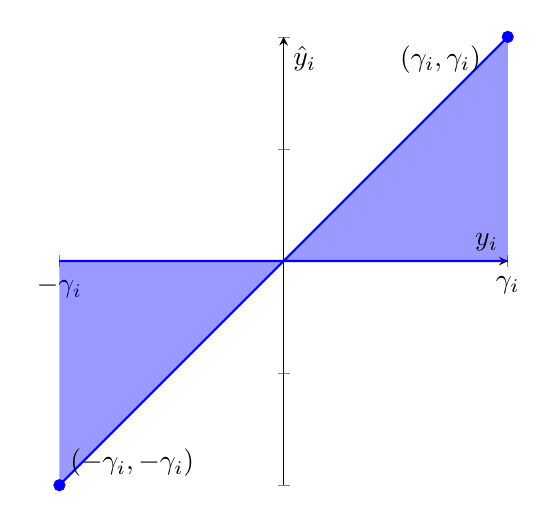
\begin{tikzpicture}
	\begin{axis}[
		xlabel={$y_i$},
		ylabel={$\hat{y}_i$},
		xmin=-2, xmax=2,
		ymin=-2, ymax=2,
		axis lines=center,
		samples=100, 
	 unit vector ratio=1 1 1, scale=1, xtick   = {-2,2},
	 xticklabels = {$-\gamma_i$,$\gamma_i$},
	 yticklabels = {},
		]
		\addplot[blue, thick, fill=blue, fill opacity=0.4] {x} \closedcycle; 
		\addplot[blue, thick] {0}; 
	
		\addplot[only marks, mark=*, mark size=2pt, blue] coordinates {(-2,-2)};
			\node[label={above:$(-\gamma_i,-\gamma_i)$}] at (axis cs: -1.35, -2.1) {};
			
				\addplot[only marks, mark=*, mark size=2pt, blue] coordinates {(2,2)};
			\node[label={above:$(\gamma_i,\gamma_i)$}] at (axis cs: 1.4, 1.5) {};
	\end{axis}
\end{tikzpicture}



The relation between $y_i$, $x'_i$ and $\hat{y}_i$ is $\hat{y}_i = \ReLU(x'_i+y_i)-\ReLU(x'_i).$ And its plots is as follows:

\hspace*{-10ex}
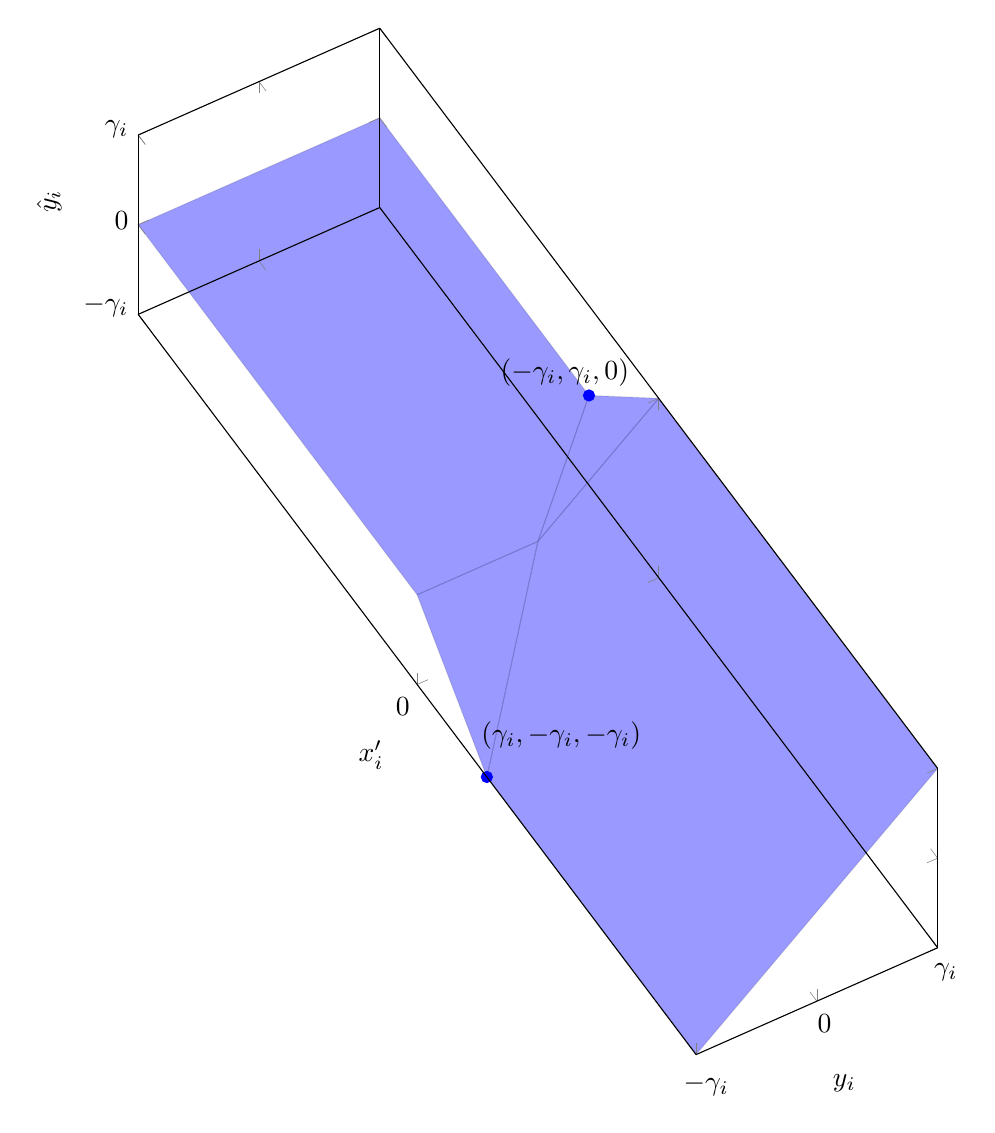
\begin{tikzpicture}
	\begin{axis}[	axis on top, xlabel = \(x'_i\),
		ylabel = {\(y_i\)}, zlabel = \(\hat{y}_i\),
				set layers=default,
	xmax = 4, xmin = -4,
ymax = 1, ymin = -1,		
zmax = 1, zmin = -1,
				unit vector ratio=1 1 1, scale=3,
				view={60}{50}, ytick   = {-1,0,1},
				yticklabels = {$-\gamma_i$,$0$,$\gamma_i$}, xtick = {0},
				xticklabels = {$0$}, ztick   = {-1,0,1},
				zticklabels = {$-\gamma_i$,$0$,$\gamma_i$},
				]
		\addplot3[fill=blue,opacity=0.1, fill opacity=0.4] 
		coordinates {
	 (0,0,0) (-1,1,0) (-4,1,0) (-4,-1,0) (0,-1,0) (0,0,0)
		};
		
		\addplot3[fill=blue,opacity=0.1, fill opacity=0.4	] 
		coordinates { (0,0,0) (0,1,1) (4, 1, 1) (4, -1, -1) (1,-1,-1) (0,0,0)
		};
		
		\addplot3[fill=blue,opacity=0.1, fill opacity=0.4	] 
		coordinates { (0,0,0)  (-1,1,0) (0,1,1) (0,0,0)
		};
		
			\addplot3[fill=blue,opacity=0.1, fill opacity=0.4	] 
		coordinates { (0,0,0)  (0,-1,0) (1,-1,-1) (0,0,0)
		};
		
		\addplot3[only marks, mark=*, mark size=2pt, blue] coordinates {(1,-1,-1)};
					\node[label={$(\gamma_i,-\gamma_i, -\gamma_i)$}] at (axis cs: 1.2, -0.5 ,-1) {};
					
			\addplot3[only marks, mark=*, mark size=2pt, blue] coordinates {(-1,1,0)};
		\node[label={$(-\gamma_i,\gamma_i, 0)$}] at (axis cs: -1, 0.8 ,0) {};			
		
	\end{axis}
\end{tikzpicture}



\hspace*{-15ex}
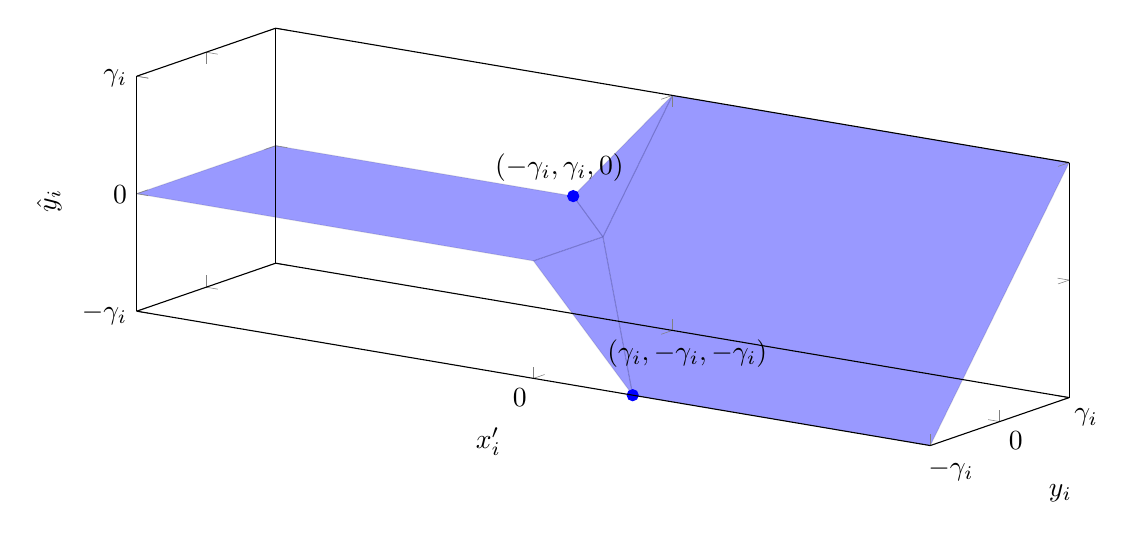
\begin{tikzpicture}
	\begin{axis}[	axis on top, xlabel = \(x'_i\),
		ylabel = {\(y_i\)}, zlabel = \(\hat{y}_i\),
		set layers=default,
				xmax = 4, xmin = -4,
		ymax = 1, ymin = -1,		
				zmax = 1, zmin = -1,
		unit vector ratio=1 1 1, scale=2.5,  ytick   = {-1,0,1},
		yticklabels = {$-\gamma_i$,$0$,$\gamma_i$}, xtick = {0},
		xticklabels = {$0$}, ztick   = {-1,0,1},
		zticklabels = {$-\gamma_i$,$0$,$\gamma_i$},
		view={35}{14},
		]
		\addplot3[ fill=blue,opacity=0.1, fill opacity=0.4] 
		coordinates {
			(0,0,0) (-1,1,0) (-4,1,0) (-4,-1,0) (0,-1,0) (0,0,0)
		};
		
		\addplot3[	fill=blue,opacity=0.1, fill opacity=0.4] 
		coordinates { (0,0,0) (0,1,1) (4, 1, 1) (4, -1, -1) (1,-1,-1) (0,0,0)
		};
		
		\addplot3[	fill=blue,opacity=0.1, fill opacity=0.4	] 
		coordinates { (0,0,0)  (-1,1,0) (0,1,1) (0,0,0)
		};
		
		\addplot3[	fill=blue,opacity=0.1, fill opacity=0.4	] 
		coordinates { (0,0,0)  (0,-1,0) (1,-1,-1) (0,0,0)
		};
		
			\addplot3[only marks, mark=*, mark size=2pt, blue] coordinates {(1,-1,-1)};
		\node[label={$(\gamma_i,-\gamma_i, -\gamma_i)$}] at (axis cs: 1.2, -0.5 ,-1) {};
		
		\addplot3[only marks, mark=*, mark size=2pt, blue] coordinates {(-1,1,0)};
		\node[label={$(-\gamma_i,\gamma_i, 0)$}] at (axis cs: -1, 0.8 ,0) {};			
		
	\end{axis}
\end{tikzpicture}


%\begin{tikzpicture}[
%	declare function={
%		f(\x,\y)=max((\x+\y),0)-max(\x,0);
%	}]
%	\begin{axis}[axis lines=center,
%		axis on top,
%		set layers=default,
%		xrange=-3:3,
%		yrange=-2:2,
%		unit vector ratio=1 1 1,% <- HERE (taken from Phelype Oleinik's deleted answer)
%		scale=3 %<- added to compensate for the downscaling
%		% resulting from unit vector ratio=1 1 1
%		]
%		\addplot3[
%		domain=-3:3,
%		domain y=-1:1, surf,
%		samples=40,
%		samples y=40,
%		] {f(\x,\y)};
%	\end{axis}
%\end{tikzpicture}




\section{Conclusion}

\newpage

\bibliographystyle{plain}
\bibliography{references}

\end{document}







\section{Ranking of Compensating Pairs}

In this subsection, we will introduce the method to choose open nodes for MILP model based on compensating pairs.

Based on No Diamond Theorem, for a target node, in its MILP model, if we open all nodes in compensating pairs, then we can get the exact values of upper and lower bound of the target node. However, in practice, this is still too expensive because we will still need to open too many nodes. So we can only choose a limited number of compensating pairs and nodes. This is by setting a parameter $O$ such that the process only choose at most $O$ many nodes to open. Therefore, in this subsection, we will introduce the process of open node chosen: given a target node, choose up to $O$ many nodes to open.


Basically, we do the process of open nodes chosen for one target node each time, that is, receive one target node (and other data) as input each time. But in principle, we can develop a method receive more than one nodes as input. But in our experiences, this does not work well.  

This process is not the unique method but the most natural way to choose open nodes. We introduce it in three steps from the simplest case to more complex case.

\subsubsection*{Value of a pair}


For a compensating pair, if $V_1,V_2$ are the values of two paths, then the value of this compensating pair is defined by: $V=\min(|V_1|,|V_2|)$.


\subsection*{Case: Source node fixed}

The simplest case is when we only consider compensating pairs with a fixed source node. 

In this case, the process is very simple: enumerate all compensating pairs, and then sort them by their values. Finally, from the first to the last compensating pair, pick all unstable nodes in its two paths except the target and source nodes into the list of open nodes, until $O$ many open nodes. 

%\subsubsection*{Sort all paths by values}
%
%The first step is to sort all paths by their values and divide paths into two groups, a group of paths with positive values and a group of paths with negative values.
%
%Since we have set a bound $O$ for open nodes, we will store  a fixed number of path for each group.
%
%\subsubsection*{Sort pairs by values}
%
%The second step is to sort all pairs by their values. Enumerate paths from the positive group and the negative group one by one and put the pairs obtained into a new list of pairs. Then sort all pair by their values from largest to the smallest: recall that the value of a pair $\langle P_1,P_2\rangle$ is $\min(|V_1|,|V_2|)$.
%
%\subsubsection*{Choosing nodes}
%
%The third step is to choose nodes from the list of pairs. According to the sorted list of pairs, enumerate pair one by one; for each pair, pick the nodes unstable in the two paths except the source and target node into the open node list. Repeat this process until $O$ nodes chosen or reach the end of the list.
%
%\subsubsection*{Pseudocode}
%
%The following needs a chart of pseudo-code
%
%\vspace*{1ex}
%
%1. Enumerate all path from the fixed source node to the target node. 
%
%2. For each path, compute its weight, that is the products of all $W_{aa'}$ along the path.
%
%3. Divide all paths into two group: positive paths and negative paths.
%
%4. Pair positive paths and negative paths from those with larger absolute values to smaller. 
%
%5. For each pair, its value is the min of the weight positive paths and absolute negative values.
%
%6. From pairs with larger values to smaller, pick path one by one, and check all intermediate nodes (nodes except source and target) of each path, and if any of them is unstable ($u>0$ and $l<0$), then open this node. 
%
%7. Repeat 6 until choosing sufficiently many nodes.
%



\subsection*{Case: Source nodes in one layer}

The more general case is when the source node can be any node in a fixed layer. In this case, the process is very similar to previous case, except the value of a pair.

In this case, for a pair $P_1,P_2$ with values $V_1,V_2$ with the source node $a$, its value is $\min(|V_1|,|V_2|)\times \text{upper bound of } a$.

%\subsubsection*{Pseudocode}
%
%The following needs a chart of pseudo-code
%
%\vspace*{1ex}
%
%1. Enumerate all path from the fixed source node to the target node. 
%
%2. For each path, compute its weight, that is the products of all $W_{aa'}$ along the path.
%
%3. Divide all paths into two group: positive paths and negative paths.
%
%4. Pair positive paths and negative paths from those with larger absolute values to smaller. 
%
%5. For each pair, its value is the min of the weight positive paths and absolute negative values, times the upper bound (at least 0) of the source node.
%
%6. From pairs with larger values to smaller, pick path one by one, and check all intermediate nodes (nodes except source and target) of each path, and if any of them is unstable ($u>0$ and $l<0$), then open this node. 
%
%7. Repeat 6 until choosing sufficiently many nodes.


\subsection*{Case: Source nodes in different layers}

The general case is that when the location of source nodes can be in different layers. This case is much more complex, because the scale level of values of paths from different layers are very different: usually a weight will be very small since every layer has a large number of nodes, therefore values of longer paths are products of more small numbers, and is definitely much smaller. If we sort all compensating pairs from different layers directly, then a very long initial segment of this list will be occupied by compensating pairs with the shortest length. Therefore, we need use some scale factors when comparing values of compensating pairs of different length.

In our experiments, we only consider the paths of length 3 (the source node is 2 layers before) and length 4 (the source node is 3 layers before). We will dynamically adjust the values during the process of node chosen. In text, the process of node chosen for length 3 plus length 4 is as follows:

\vspace*{1ex}

1. Generate the two lists of pairs sorted by their values for source nodes in 2 layers before the target node and 3 layers before separately as in the previous case.

2. Enumerate pair from two lists one by one by their values and pick nodes as previous case. When comparing the values between pairs of length 4 and pairs of length 3, multiply the numbers of nodes in 1 layer before to the value of pair of length 4.

In formula, when the target node is in layer $L$, for a pair $P_3$ of length 3 with value $V_3$ and a pair $P_4$ of length 4 with value $V_4$, if we have chosen $N$ nodes in layer $L-1$. Then the adjusted values for $P_3$ and $P_4$ are: $$V_3, N\cdot V_4.$$ Then we pick the next pair by the adjust value in two lists.

3. Repeat 2 until choosing sufficiently many nodes.

\vspace*{1ex}

The pseudo-code is as follows ():

\begin{algorithm}
\caption{Process for length 3 + length 4}
\KwData{Sorted lists of length 3 + length 4}
\KwResult{Open node list}

Let $N = 0$ be the number of Chosen length 4 pair.

\While{len(Open node) $<O$}{
	Pick the first element $P_3$ in the list of length 3\;
	
	Let $V_3$ be the value of $P_3$\;
	
	Pick the first element $P_4$ in the list of length 4\;
	
	Let $V_4$ be the value of $P_4$\;
	
	\If{$V_3 > V_4 \cdot N$}{
		Add nodes in $P_3$ into Open list\;
		Number of Chosen lentgh pair $N$ += 1\; 
	}
	\Else{
		Add nodes in $P_4$ into Open list\;
	}
}
\end{algorithm}



\end{document}


